%-/`-/`-/`-/`-/`-/`-/`-/`-/`-/`-/`-/`-/`-/`-/`-/`-/`-/`-%
% CS 196 Copyrights and Patents Survey
% 
% Typeset with the `acmlarge` template by Donald Knuth & Leslie Lamport
% 
% Copyright 2016 Fiestada, Lobaton, Dacuba, Cañedo, Latoga
% For more information about this survey, go to https://cs196copyrights.github.io/survey
% or email the Git repo maintainer at vffiestada@up.edu.ph
%
%-/`-/`-/`-/`-/`-/`-/`-/`-/`-/`-/`-/`-/`-/`-/`-/`-/`-/`-%
\documentclass[prodmode,cs196]{acmlarge}

\usepackage{float}
\usepackage{bchart}
\usepackage{pgf-pie}

% Metadata Information
\acmVolume{1}
\acmNumber{1}
\acmArticle{2}
\articleSeq{1}
\acmYear{2016}
\acmMonth{09}

% Page heads
\markboth{Ca\~{n}edo, Dacuba, Fiestada, Latoga, and Lobaton}{Opinions of UP Diliman Students on Technology Copyrights and Patents}

% Title portion
\title{Opinions of UP Diliman Students on Technology Copyrights and Patents}
\author{ABBY CA\~{N}EDO, CARISSE DACUBA, VINCENT FIESTADA, AREL LATOGA, and TROI LOBATON \affil{University of the Philippines Diliman}}

\begin{abstract}
In this paper, the authors take a look at the popular opinion of Science and Engineering majors in the University of the Philippines Diliman Students regarding isssues around technological copyrights and patents. In particular, this paper examines their opinions on the extent of influence that a particular piece of design or feature has on a whole product. This is done in the context of the Samsung vs. Apple and Oracle vs. Google trials over the infringement of intellectual property rights.
\end{abstract}

\category{Ethical and Professional Issues}{Technology and Computing}{Popular views and opinions}[Surveys and Analyses]

\terms{Patents \and Copyrights}
\keywords{Ethics, patents, copyrights, technology, computing}

\acmformat{Ca\~{n}edo, Dacuba, Fiestada, Latoga, and Lobaton. 2016. Opinions of UP Diliman students on technology copyrights and patents.}

\begin{document}

\begin{bottomstuff}
\copyright Copyright 2016 Ca\~{n}edo, Dacuba, Fiestada, Latoga, and Lobaton.
\end{bottomstuff}


\maketitle

\section{Introduction}

Technological patents and copyrights pose an important issue for software developers, hardware manufacturers, designers, and other stakeholders in the technology industry and those communities concerned about technological proliferation. These issues raise questions about how much control an entity should have over its creation, what protections should be afforded that entity, and how those protections should be balanced to still allow continued innovation in the field. Furthermore, how much influence does a particular piece of design or technology have over a product? 

\subsection{Intellectual Property Rights}

Intellectual property (IP) such as art, designs, and inventions are identified as non-physical works that are the "product of original thought". Rights can be granted to the owners of IP. These rights cover the control of the expressions of IP (such as physical expressions in the form of manufactured products, or digital copies of a work of art or piece of technology). Intellectual property rights protects the interests of the creator by giving them control over the production and distribution of expressions of their work. \cite{MooreHimmaIP} Protections can be granted by law in the form trademarks, trade secrets, patents, and copyrights. This paper is concerned with the latter two.

A patent is a set of rights given to the owner of an invention that prevents others from making, using, importing, or selling the invention without the owner's permission. To be patented, an invention must be "new, an improvement over current processes or technologies, and must have practical industrial application". \cite{IPOSPatent} 

In general, patents expire (currently, the expire after 15 years in the US), but since the allegations discussed here fall within the time frame, a description of patent time limits can be safely ommitted. Most countries grant patents to several types of intellectual property. This paper is generally concerned with design and utility patents. 

In the United States, where the Apple patents were filed, a design patent can be applied for the ornamental or aesthetic design of a product, including its physical properties and appearance. Patents last for 15 years in the US and allows its holder to disallow the unauthorized use, marketing, or selling of a design. \cite{USPTOPatents}

A utility patent is one granted to a useful and novel, or previously unknown, process, machine, manufactured product, or composition of matter. These include the patent granted for Samsung's wireless technologies. \cite{USPTOPatents}

A copyright constitutes a different set of rights granted to an intellectual property owner. They are the legal rights given to the creator of works such as writings, paintings, photographs, and computer programs--i.e. expressions of ideas. Copyright prevents others from reproducing, distributing, creating derivatives from, and displaying the work in public. Another important distinction between copyright and patents is that while patents have to be applied for, copyright automatically applies to all copyrightable material. \cite{PlagiarismTodayCopyright}

\subsection{Apple vs. Samsung}

\textbf{Apple vs. Samsung} is a series of patent infringement lawsuits filed by Apple Inc. and Samsung Electronics Corp. against each other. As of the time of this writing, some cases are still pending in several courts. Apple has several design patents, including patents for the iPhone's shape, the colors of the graphical user interface of iOS, and the shape and design of the iPad.

%% Photographs from Apple's design patents
\begin{figure}[H]
	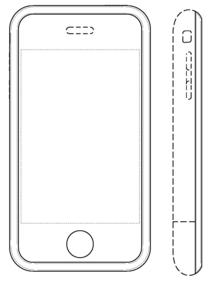
\includegraphics[width=0.3\textwidth]{apple_iphone_shape.png}
	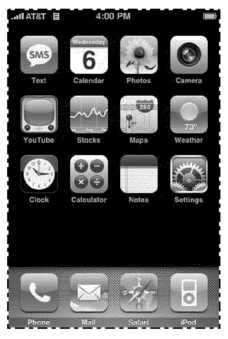
\includegraphics[width=0.3\textwidth]{apple_iphone_icons.png}
	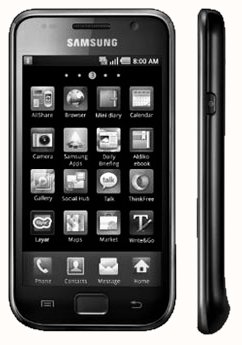
\includegraphics[width=0.3\textwidth]{samsung-galaxy-i9000.png}
	\caption{From the left: a) A front and side profile of Apple's iPhone according to the US patent grant for its design; b) A screenshot of the home screen of the iPhone showing the patented user interface; c) A front and side profile with the home screen of the Samsung Galaxy i9000, claimed by Apple to be an infringement of its design patents. }
\end{figure}

On April 15, 2011, Apple sued Samsung in the United States District Court for the Northern District of California, claiming that Samsung infringed on Apple's patents. A few days later, on April 22, Samsung counter-sued Apple in the federal courts of Seoul, South Korea; Tokyo, Japan; and Mannheim, Germany, claiming that Apple infringed upon its own patents on wireless technology.

Seoul found infringements against Samsung and Apple, ordering the ban from sales of the infringing products. Tokyo ruled in favor of Samsung, and awarded Samsung reimbursement for the legal costs. Mannheim ruled in favor of Apple, ordering the sales ban on Galaxy Tab 10.1.

In the United States courts, Apple cited the similarities between its own iPhone and iPad products and the Samsung Galaxy line of smartphones and tablets. In particular, Apple claimed infringement of US D593087 (for the "home button, rounded corners, and tapered edges" of the iPhone); \cite{AppleiPhoneDesignPatent} against Samsung’s Samsung Galaxy i9000. Another design patent infringement claimed by Apple against Samsung was US D604305, which was Apple’s “On Screen Buttons”. \cite{anzures2009graphical} The court again ruled in favor of Apple. Lastly, another design patent infringement claimed by Apple against was US D504889, which is the patent for Apple’s iPad. \cite{andre2005electronic}

Besides design patents, Apple also sued Samsung for utility patents, such as Apple’s “Bounce Back” feature, or the “Slide to Unlock” feature.

All of the above infringements were included in the first trial in the United States. Although injunctions for sales ban against the infringing products were ordered, eventually it was reversed, but in a retrial for damages, Apple was awarded US\$290 million.

The battle bounces back and forth, with one side winning a case and being awarded with damages and vice versa. For some, the patent war may be about the money, but for Samsung and Apple, it was “a fight over invention and copying and for the reputation as an innovator.” \cite{CNet}

\subsection{Oracle vs. Google}

\textbf{Oracle vs Google} was a dispute between the owners of Java (Oracle America, Inc.) and Android (Google, Inc.). Java is a programming language and set of libraries that was created by Sun Microsystems. Included with Java was an Application Programming Interface, which is a set of software tools that are meant to be used by other software to achieve a certain functionality. \cite{Sintes2001} The Java API allowed programmers to simplify their code and rely on existing libraries instead.

Android was created by Android, Inc. and was later bought and further developed by Google. At an early stage of development, it was announced that it would use Java technologies. At the time, Sun Microsystems publicly praised the decision, with then CEO Jonathan Schwartz "offering my heartfelt congratulations to Google on the announcement of their new Java/Linux phone platform, Android." \cite{Schwartz2007} Google's own implementation of Java APIs were included in the Android Software Development Kit, which was an instrumental tool in allowing developers to write apps that would extend the functionality of Android.

Sun Microsystems was bought by Oracle in 2010, while Android became one of the most used operating systems in the world. In August 2010, Oracle sued Google, claiming that Google violated infringed on its intellectual property when it created its own version of the Java API and demanded payment for damages. In its initial complaint, Oracle accussed Google of "knowingly, willingly, and unlawfully" copying, using, and redistributing its IP without express permission. \cite{Bangeman2003}. 

There were several stages of the litigation process, characterized by three major decisions subsequently handed down by different courts. These decisions and the reasons for them are presented in the following figure.

\begin{figure}[H]
	\begin{tabular}{|p{0.3\textwidth}|p{0.3\textwidth}|p{0.3\textwidth}|}
		\hline
		\textbf{Ruling} & \textbf{Winner} & \textbf{Notes} \\
		\hline
		The APIs that Google "copied" were not protected by copyright & Google & The court reasoned that if \quote{there is only one way to declare a given method functionality, [so that] everyone using that function must write that specific line of code in the same way"}.\\
		\hline
		A higher court reversed the ruling; the Java APIs are protected by copyright & Oracle & \\
		\hline
		Google's use of them was under the terms of fair use & Google & The ruling that the Java APIs are protected by copyright still stands\\
		\hline 
	\end{tabular}
	\caption{Listing of subsequent rulings at different stages of the litigation process between Oracle and Google. Google's defense was originally based on the triviality of the parts that were copied from the Java APIs, then the uncopyrightability of APIs, but in the end were forced to retreat and use a fair use defense.}
\end{figure}

Oracle had demanded financial compensation for Google's alleged violations, seeking up to US 9.3 billion dollars during its second trial. This was close to 4 billion dollars more than Oracle had paid for Sun Microsystems, and was at the time the largest amount demanded for an IP settlement. Oracle claimed that it deserved all of the profits made from Android because if it wasn't for Java, Android could not have competed during the early days of its depolyment. It cited how Google capitalized upon the wide market share of Java and used it to attract developers their then-fledgling platform. Google maintained that compensation, if any at all, paid to Oracle should have been much lower.\cite{Mullin2016}

Many computer scientists disputed the second ruling, which reversed the initial decision that APIs were not protected by copyright. In an amicus brief filed by the Electronic Fronteir Foundation on behalf of computer scientists, they petitioned the court to favor the first ruling. Many in the software industry agreed with the fair use ruling, but still believed that the APIs should not have been copyrighted in the first place, obfuscating the need to go through trials in the first place. \cite{EFFAmicusBrief}

Other groups such as the Picture Archive Council of America and Graphic Artists Guild argued against Google's fair use defense. They cited that it was "not fair" that Google used the creative works of Oracle to jump-start their venture into a new and lucrative field. They also maintained that court's third decision undermined the copyrights not only in software, but in all forms of creative works. \cite{ProOracleAmicusBrief}

\section{Objectives}

This survey is undertaken with the objectives

\begin{itemize}
	\item{to determine the familiarity of UP Diliman Engineering and Science undergraduates with the patent and copyright infringement lawsuits between Apple \& Samsung; and Oracle \& Google, respectively;}
	\item{to determine the prevailing opinion of UP Diliman Engineering and Science undergraduates about the validity of Apple's infringement claims against Samsung;}
	\item{to determine the prevailing opinion of UP Diliman Engineering and Science undergraduates about the validity of Oracle's infringement claims against Google;}
	\item{to determine the likely response of UP Diliman Engineering and Science undergraduates to an infringement of their own intellectual property;}
\end{itemize}

\section{Methodology}

The survey was carried out over a sample of undergraduate students in the University of the Philippines Diliman campus pursuing engineering and science degrees. Opportunistic sampling was used to select participants. Respondents were asked to answer thirteen (13) Yes/No questions, and 2 other multiple choice questions; the questionnaire pertained to their familiarity with the Apple vs. Samsung and Oracle vs. Google cases, the products (namely, the iPhone, iPad, Galaxy phones and tablets, Java and Android), perceptions about the correctness of major court decisions handed down during the course of the litigation processes, and what they would do in the case of their own intellectual property being infringed upon and used for profitable purposes. Regarding that same situation, they were asked if they would demand a stop to distribution/manufacture of the infringing product and what amount of the violators' profits they would demand as compensation (none, some or all).

The questionnaires were administered either online or via paper forms, and also included briefing information about the cases, images of the products in question (where relevant), and definition of legal and technical terms pertaining to the cases. The entire questionnaire is available at the project site (please see the footnotes in the first page of this paper).

\section{Results and Discussion}

The respondents interviewed had a fair amount of familiarity with the products in question (iPhones, iPads, Galaxy phones and tablets, Java and Android). The data also showed a large overlap over the familiarity of respondents. Many respondents were familiar with several of the products, with around 55\% being familiar with all of them.

\begin{figure}[H]
	\begin{bchart}[min=0, step=10 ,max=100]
		\bcbar[text="iPhones \& iPads", color=purple!30]{92.22}
            \smallskip
        \bcbar[text="Galaxy phones \& tablets", color=blue!50]{83.33}
            \smallskip
        \bcbar[text="Java", color=yellow]{61.11}
			\smallskip
        \bcbar[text="Android", color=green]{93.33}
    \end{bchart}
	\caption{Percentages of respondents who were familiar with the products involved in the court cases in question.}
\end{figure}

\subsection{Opinions on Apple vs. Samsung}

Respondents were asked Yes/No questions about their opinions of the court decisions on the Apple vs. Samsung trials. 40\% of respondents already knew of the case beforehand, while 60\% did not.

\begin{figure}[H]
	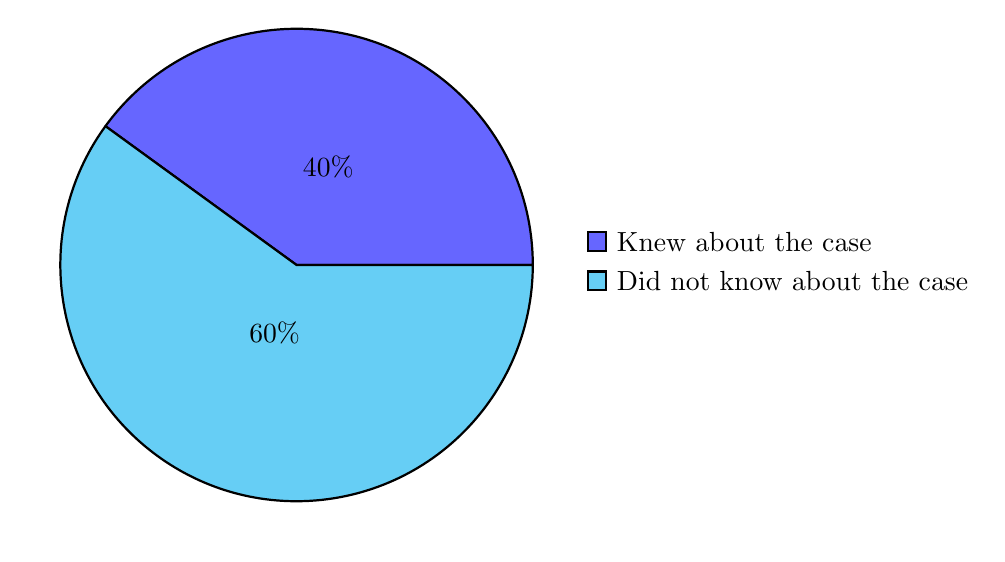
\begin{tikzpicture}
		\pie[text=legend]{40/Knew about the case, 
			  60/Did not know about the case}
	\end{tikzpicture}
	\caption{Percentage of respondents who knew about the Apple vs. Samsung series of cases.}
\end{figure}


As to the charges of infringement upon Apple's design patents, 67\% thought that Samsung was \textbf{not guilty} of infringing upon Apple's patent for the ornamental design of the iPhone. 62\% of respondents thought that Samsung was \textbf{not guilty} of infringing upon Apple's patent for on-screen icons. 78\% of respondents agreed that Samsung was \textbf{not guilty} of violating Apple's iPad patents.

\begin{figure}[h]
	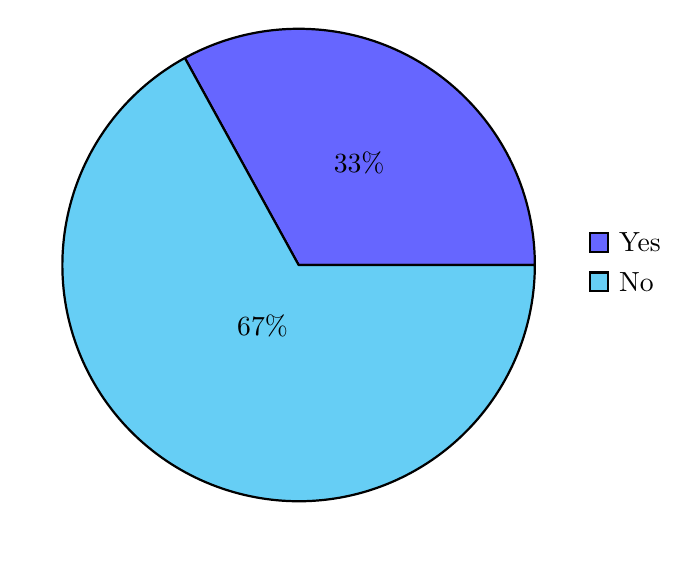
\begin{tikzpicture}
		\pie[text=legend]{33/Yes, 
			  67/No}
	\end{tikzpicture}
	\caption{Respondents' answers to "Samsung was found guilty of infringing Apple’s design patent of “home button, rounded corners and tapered edges (US D593087)” (See picture for comparison). Do you agree with the decision?"}
\end{figure}

\begin{figure}[h]
	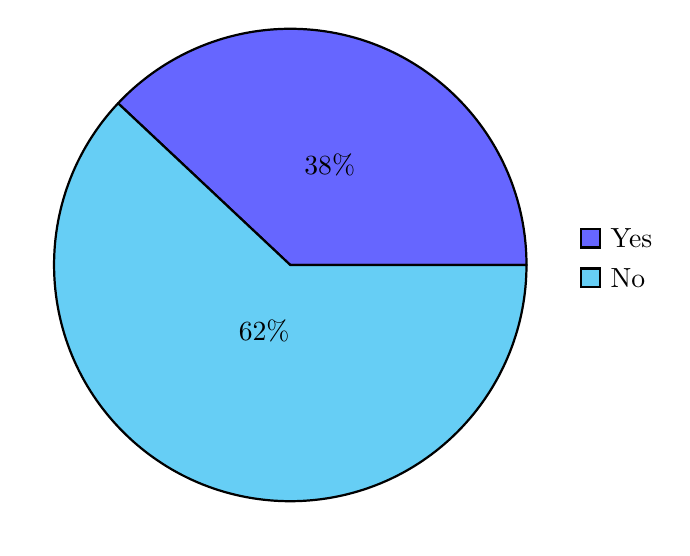
\begin{tikzpicture}
		\pie[text=legend]{38/Yes, 
			  62/No}
	\end{tikzpicture}
	\caption{Respondents' answers to "Samsung was found guilty of infringing Apple’s design patent of “On-Screen Icons  (US D604305)” (See picture for comparison). Do you agree with the decision?"}
\end{figure}

\begin{figure}[H]
	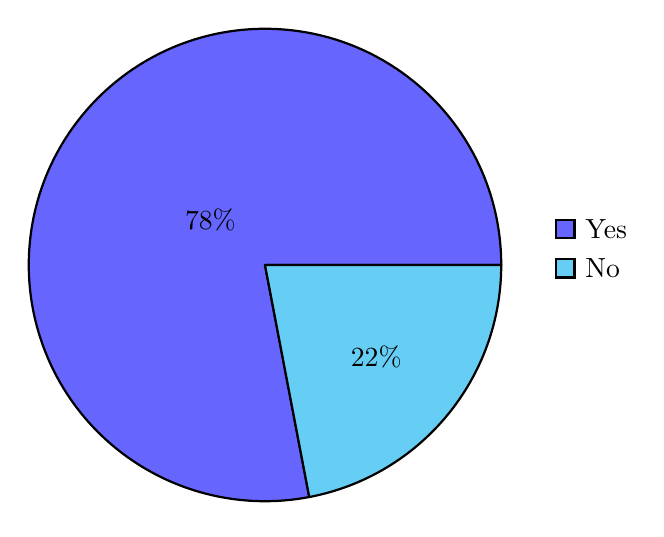
\begin{tikzpicture}
		\pie[text=legend]{78/Yes, 
			  22/No}
	\end{tikzpicture}
	\caption{Respondents' answers to "Samsung was found not guilty of infringing Apple’s design patent for their iPad (US D504889) (See picture for comparison). Do you agree with the decision?"}
\end{figure}

In regards to the amicus briefs delivered by various third parties, 76\% of respondents agreed with the amicus brief from Dell, Facebook, Google and others that a patent infringement should not be worth the entire product. However, 63\% agreed with the opposing amicus brief that it is the design that sells and makes profit for a product.

\begin{figure}[h]
	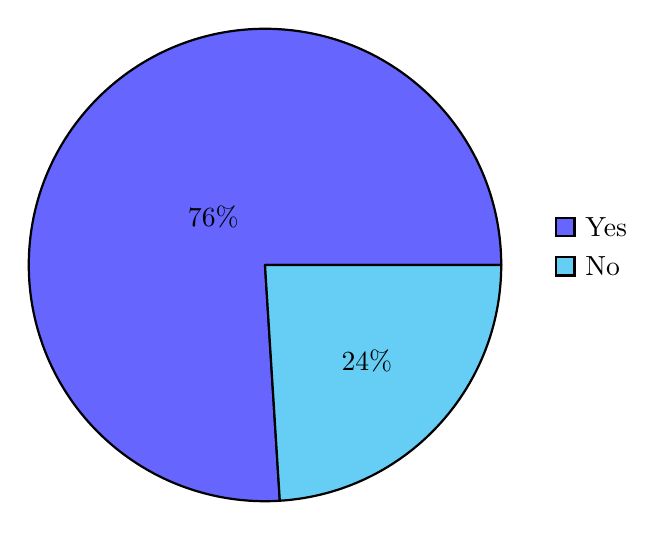
\begin{tikzpicture}
		\pie[text=legend]{76/Yes, 
			  24/No}
	\end{tikzpicture}
	\caption{Respondents' answers to whether they agreed with an amicus brief saying that "a patent infringement should not be worth the entire product."}
\end{figure}

\begin{figure}[H]
	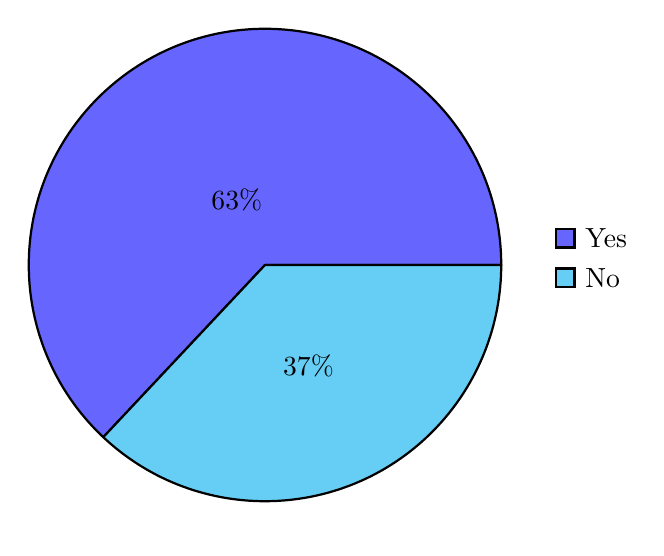
\begin{tikzpicture}
		\pie[text=legend]{63/Yes, 
			  37/No}
	\end{tikzpicture}
	\caption{Respondents' answers when asked whether "design sells the product, and it is what makes profit for the product".}
\end{figure}

Interestingly enough, 42\% of respondents agreed with both amicus briefs. The divide of respondents who agreed with only one of the amicus briefs was fairly even. 34\% agreed with only the second amicus brief (that the design sells the product) and  21\% agreed with only the first amicus brief (that a patent infringement should not be worth the whole product). All in all, it seems that most of the respondents sided with Samsung but could not completely abandon the idea that a design plays a large role in the perception and success of a product.

\subsection{Opinions on Oracle vs. Google}

Overwhelmingly, most respondents (93\%) were not previously aware of the case between Oracle and Google. This might just be because this case has not been as extensively covered by the media, and because the products involved (Java and the Andrioid SDK) are more targeted at developers, and so are not under general consumer scrutiny. This may also tie back to the relatively low number of respondents who were familiar with Java, even though most were familiar with Android.

\begin{figure}[h]
	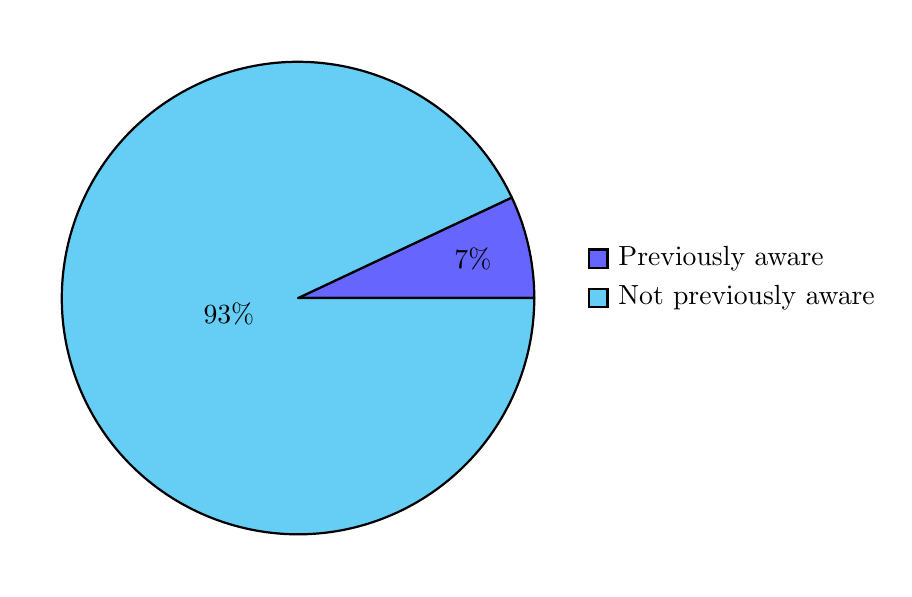
\begin{tikzpicture}
		\pie[text=legend]{7/Previously aware, 
			  93/Not previously aware}
	\end{tikzpicture}
	\caption{Percentage of Respondents who were previously aware of the case between Oracle and Google.}
\end{figure}

Only 52\% of respondents agreed with the initial court decision, that APIs do not contain any expressiveness or creativity and are therefore not protected by copyright. 49\% agreed with the second ruling, that the Java API should be protected by copyright. 81\% agreed with the third ruling, that Google's use of the Java APIs were under fair use. The respondents appear to be more evenly split about this issue and seem reluctant to penalize any one side.

\begin{figure}[h]
	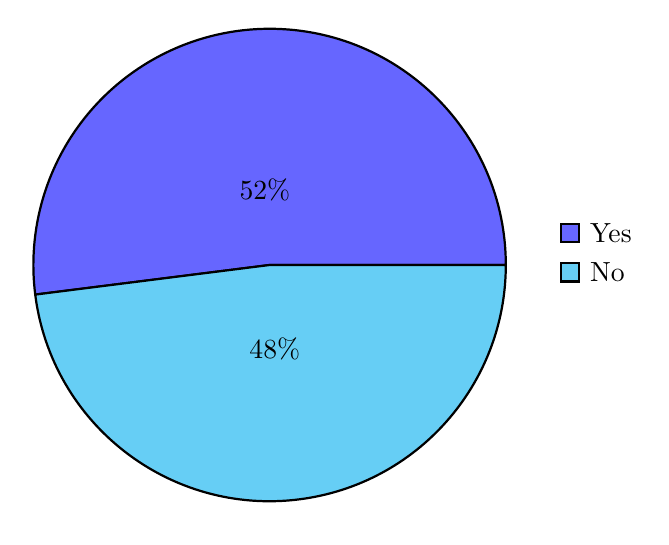
\begin{tikzpicture}
		\pie[text=legend]{52/Yes, 
			  48/No}
	\end{tikzpicture}
	\caption{Respondents' answers to "APIs were declared to be free of copyright because it was considered too generic and reflected the only functional way to do something...APIs do not contain any expressiveness or creativity. Do you agree?"}
\end{figure}

\begin{figure}[h]
	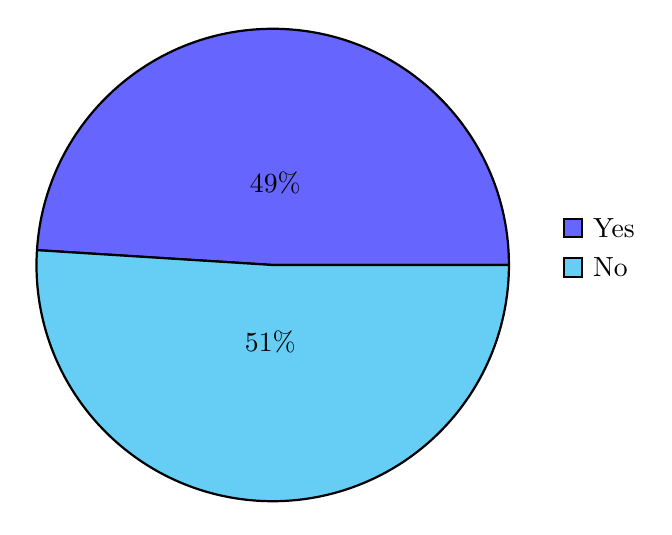
\begin{tikzpicture}
		\pie[text=legend]{49/Yes, 
			  51/No}
	\end{tikzpicture}
	\caption{Respondents' answers to "The second ruling reversed the first one, declaring that the Java API was protected by copyright. Do you agree?"}
\end{figure}

\begin{figure}[H]
	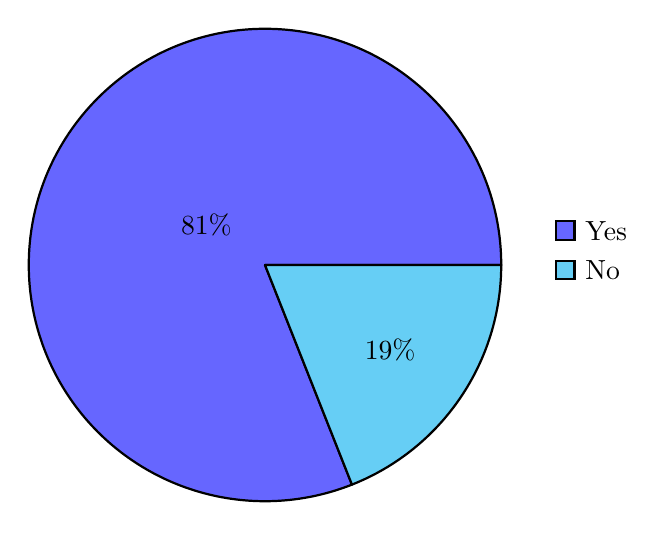
\begin{tikzpicture}
		\pie[text=legend]{81/Yes, 
			  19/No}
	\end{tikzpicture}
	\caption{Respondents' answers to "The third ruling defended Google’s use of the Java API as fair use, ensuring that the copyright laws could not hinder innovations made by Google. Do you agree that it was fair use?"}
\end{figure}

Meanwhile, 74\% of respondents agreed with the amicus brief filed by the EFF, and that APIs should not be copyright-protected. Only 46\% agreed with the second amicus brief, and that copying Oracle's IP to jump-start a lucrative venture was not fair use. 46\% of respondents agreed with the first amicus brief and did not agree with the second. Only 18\% of respondents agreed with the second but not the first amicus brief. All in all, the respondents seem to be fairly evenly split on this issue, but with those in favor of Google and the EFF's side having a slight edge, especially when exclusivity of stance is taken into account.

\begin{figure}[h]
	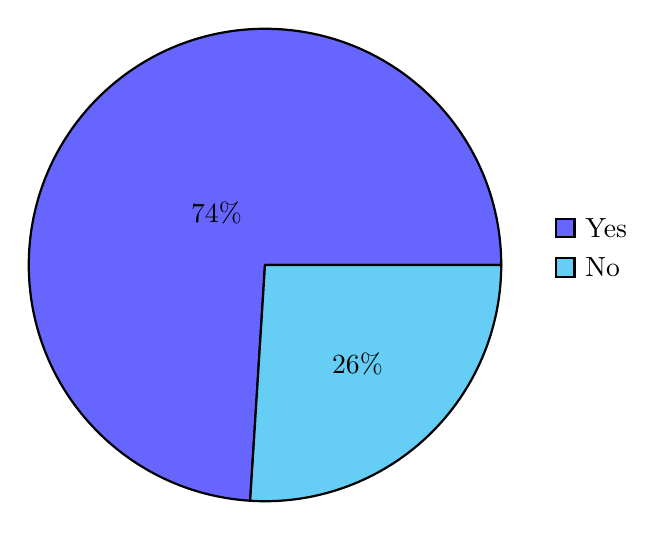
\begin{tikzpicture}
		\pie[text=legend]{74/Yes, 
			  26/No}
	\end{tikzpicture}
	\caption{Respondents' answers to "...Many in the software industry agree with the fair use ruling, but still believe that APIs shouldn’t be copyright-protected in the first place. Do you agree with them?"}
\end{figure}

\begin{figure}[H]
	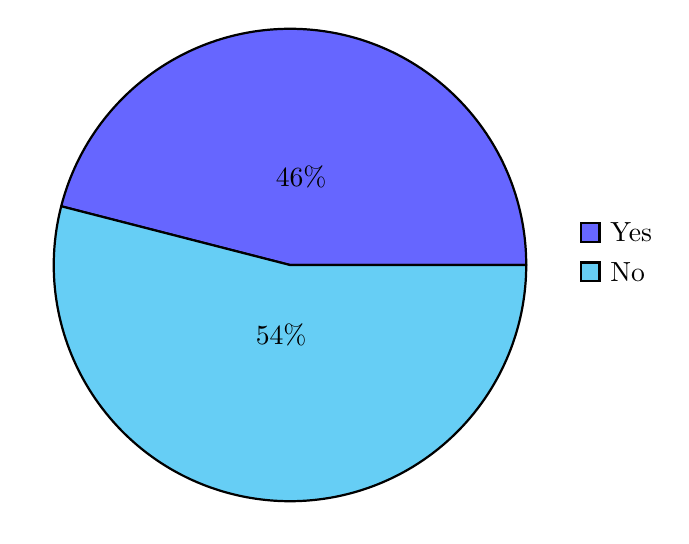
\begin{tikzpicture}
		\pie[text=legend]{46/Yes, 
			  54/No}
	\end{tikzpicture}
	\caption{Respondents' answers when asked whether they agreed to the amicus brief saying "it was not “fair” that Google used the creative works of Oracle to jump start their venture into a new and lucrative field."}
\end{figure}

\subsection{General Opinions}

For the last pair of questions, respondents were presented with a situation that pertains to their stance on intellectual property control in general. When asked whether they would demand a stop to someone who created a popular and profitable product using part of their work, 54\% said yes. In the same situation, 80\% of respondents said that they would demand for a portion (but not all) of the profits made from the infringing product.

\begin{figure}[h]
	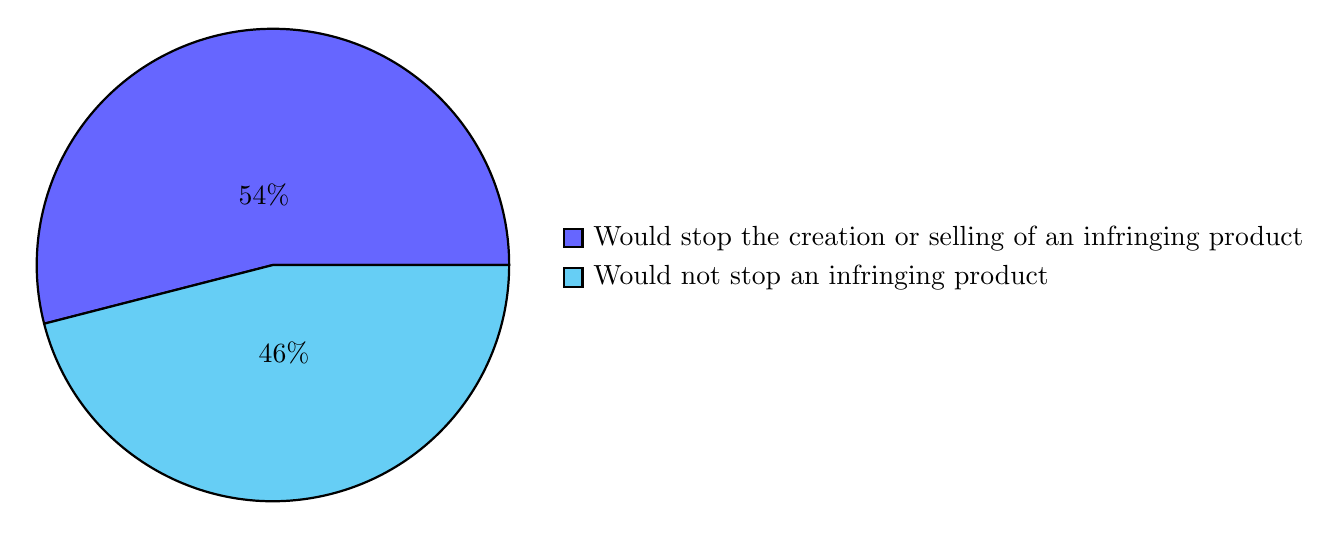
\begin{tikzpicture}
		\pie[text=legend]{54/Would stop the creation or selling of an infringing product, 
			  46/Would not stop an infringing product}
	\end{tikzpicture}
	\caption{Respondents' hypothetical actions in response to a product that infringed upon their work.}
\end{figure}

\begin{figure}[H]
	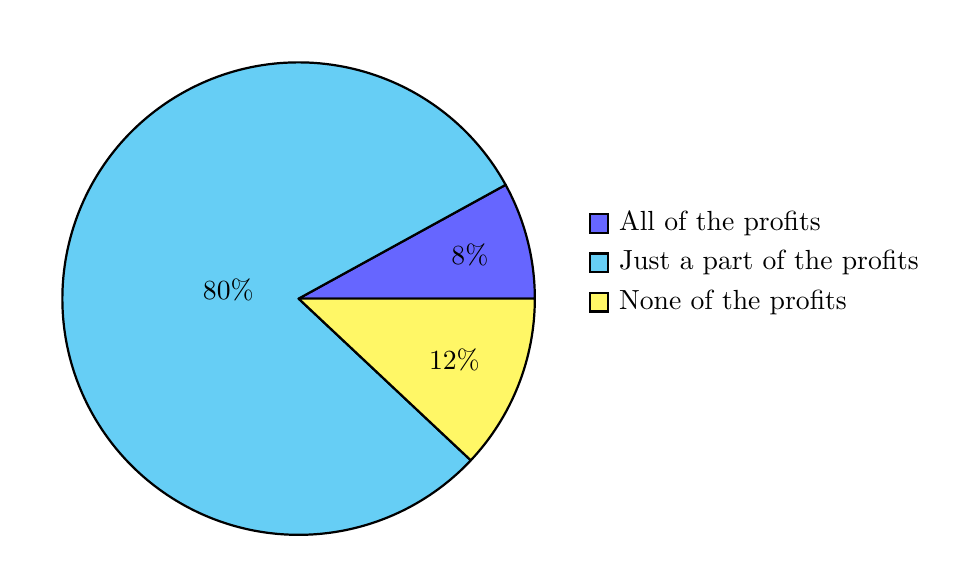
\begin{tikzpicture}
		\pie[text=legend]{8/All of the profits, 
			  80/Just a part of the profits,
			  12/None of the profits}
	\end{tikzpicture}
	\caption{Respondents' answers when asked what they would ask for as compensation from an infringing party.}
\end{figure}

While it seems that the data is unclear in some areas (as respondents seem to find it difficult to side completely with one party), a pattern can be seen to arise from the results. In the case of Apple vs. Samsung, respondents seem to favor Samsung and attest for the most part that is not guilty of infringement. However, they are also divided on the issue of how much design plays a role in the product, simulataneously attesting that an infringement of parts of a product is not worth the entire product, as well as the design playing a major role in creating value for a product.

In the case of Oracle vs. Google, popular opinion seems to be more lukewarm. This may be because of little previous knowledge about the case. However, those in favor of the side of Google and the EFF seem to have a slight but still significant edge. Many respondents agreed that Google was under fair use (81\%) and only 18\% agreed with the second amicus brief exclusively, which said that Google was \textit{not} under fair use.

Most respondents would also stop the creation or distribution of an infringing work (although the difference here is not that vast). But a large majority of respondents believe that compensation for infringement should only be part of the profits, and not all of it.

\section{Conclusion}

Opinion appears to be that patents and copyrights should be uphelpd (hence their agreement that Apple's design created value for the product and the lukewarm support of Google). However, as demonstrated by their support of fair use, the large minority of people who would not stop an infringing product, and the overwhelming desire to ask only for part of (but not all) of the profits as compensation--these factors may be viewed as evidence that the students believe that an infringing produc may still have value that is independent of what is copied, and that punishments for violators should not be so extreme that it diminishes that amount of work put into a product by the infringing party.

In summary, it the recommendation of the authors that popular opinion in the target demographics to be: intellectual property rights should be upheld and the work of original creators acknowledged, but not at the expense of potential innovations made by third parties. Furthermore, when a work is infringed upon, the transformative nature of the infringing work should not be ignored or diminished.

\nocite{AppleiPhoneDesignPatent}

\label{sect:bib}
\bibliographystyle{acmref}
\bibliography{report_sources}{}

\end{document}